\documentclass[12pts]{report}
\usepackage{xcolor, colortbl}
\usepackage{algorithm}
\usepackage[noend]{algpseudocode}
\usepackage{textcomp}
\usepackage{listings}
\usepackage{hyperref}
\usepackage{alltt}
\usepackage{tikz}
\usepackage{framed}
\usepackage{mdframed}
\usepackage{marvosym}
\usepackage{wasysym}
\usepackage{marvosym}
\usepackage{crayola}
\usepackage{mathpartir}
\usepackage{tabularx}
\usepackage[belowskip=-15pt,aboveskip=0pt]{caption}
\usepackage[skins]{tcolorbox}
\usepackage{multicol}
\usetikzlibrary{positioning,shapes,arrows, backgrounds, fit, shadows}
\usetikzlibrary{arrows.meta}
\usetikzlibrary{decorations.markings}
\usepackage[margin=1in]{geometry}

\newcommand{\kcquestion}[1]{
\begin{framed}
{\noindent\color{BrickRed}Q:} #1
\end{framed}
}

\newcommand{\kcbox}[2]{
	\vspace{1cm}
	\begin{minipage}{\textwidth}
		\begin{mdframed}[backgroundcolor=OliveGreen!20] 
			\begin{center}
				\underline{\textsc{\color{Brown}#1}}
			\end{center}
		
			{#2}

	    \end{mdframed}
	\end{minipage}
}

\newcommand{\pendingtopic}[1]{
\textbf{\color{Red}#1}
}
\tikzstyle{bb}=[%
      rectangle, draw=black, thick, fill=OliveGreen!30, drop shadow, align=center,
      text ragged, minimum height=2em, minimum width=2em, inner sep=6pt
]

\tikzstyle{inv}=[%
      rectangle, draw=none,  align=center,
      text ragged, minimum height=2em, minimum width=2em, inner sep=6pt
]

\tikzstyle{db}=[%
      ellipse, draw=black, thick, fill=pink, drop shadow, align=center,
      text ragged, minimum height=2em, inner sep=6pt
]

\tikzstyle{jn}=[%
      ellipse, draw=black, thick, fill=black
]

\tikzstyle{io}=[%
      trapezium, trapezium left angle=60, trapezium right angle=120, draw=black, thick, fill=brown, drop shadow,
      text ragged, minimum height=2em, minimum width=2em, inner sep=6pt, align=center
]

\tikzstyle{glio}=[%
      trapezium, trapezium left angle=60, trapezium right angle=120, draw=red, line width = 1mm, fill=brown, drop shadow,
      text ragged, minimum height=2em, minimum width=2em, inner sep=6pt
]
\tikzstyle{gl}=[%
      rectangle, draw=red, line width = 1mm, fill=lightblue, drop shadow,
      text ragged, minimum height=2em, minimum width=2em, inner sep=6pt
]

\tikzstyle{en}=[%
      rectangle, draw=black, thick, fill=none,
      text ragged, minimum height=2em, minimum width=2em, inner sep=6pt
]

\tikzstyle{sh}=[%
      rectangle, draw=gray, thick, fill=none, color = gray,
      text ragged, minimum height=2em, minimum width=2em, inner sep=6pt
]

\tikzset{obj/.style = {rectangle split, rounded corners,
                      rectangle split parts=2, very thick,draw=black!50, top
                      color=white,bottom color=black!20, align=center}}

\tikzset{cobj/.style = {rectangle split,
                      rectangle split parts=3, very thick,draw=black!50, top
                      color=white,bottom color=black!10, align=left}}

\lstset{
	language = java,
	basicstyle = \ttfamily\small,
	stringstyle = \ttfamily,
	keywordstyle=\color{Blue}\bfseries,
	identifierstyle=\color{Pink},
	commentstyle=\color{OliveGreen},
	frameround=tttt,
	showstringspaces=false,
	captionpos=b
}
\lstdefinestyle{pc}{
	language = Python,
	basicstyle = \ttfamily,
	stringstyle = \ttfamily,
	keywordstyle=\color{Blue}\bfseries,
	identifierstyle=\color{Pink},
	commentstyle=\color{Green},
	frameround=tttt,
	frame=single,
%	numbers=left
	showstringspaces=false
}

\lstdefinestyle{jc}{
	language = Java,
	basicstyle = \ttfamily\small,
	stringstyle = \ttfamily,
	keywordstyle=\color{Blue}\bfseries,
	identifierstyle=\color{Pink},
	commentstyle=\color{Green},
	frameround=tttt,
%	numbers=left
	showstringspaces=false
}

\lstdefinestyle{cc}{
	language = Caml,
	basicstyle = \tiny\ttfamily,
	stringstyle = \color{red}\ttfamily,
	keywordstyle=\color{Blue}\bfseries,
	identifierstyle=\ttfamily,
	frameround=tttt,
	numbers=none,
	showstringspaces=false,
	escapeinside={(*@}{@*)}
}

\lstdefinestyle{oc}{
	language = bash,
	backgroundcolor = \color{Black!70},
	basicstyle = \small\ttfamily\color{white},
	stringstyle = \color{red}\ttfamily,
	keywordstyle=\color{white}\bfseries,
	identifierstyle=\ttfamily,
	frameround=tttt,
	numbers=none,
	showstringspaces=false,
	escapeinside={(*@}{@*)}
}

\author{Sujit Kumar Chakrabarti}
\title{A Basic Test Automation Set-up}

\begin{document}
\maketitle
\chapter{Introduction}
\section{Program under test (PUT) - Jugs}

The program under test is a solution to a simple programming puzzle: Given
two jugs of capacity c1 and c2, and a final volume f, the program should
find the shortest sequence of steps to be followed to achieve a volume of
f in either of the jugs the other being empty.


\chapter{Test Execution Automation}
\section{Instructions for Use}
To compile the Jugs program, run:
\begin{lstlisting}[style=oc]
	make jugs
\end{lstlisting}

To run the Jugs program, run:
\begin{lstlisting}[style=oc]
	./jugs c1 c2 f
\end{lstlisting}

For example, running:
\begin{lstlisting}[style=oc]
	./jugs 9 15 3
\end{lstlisting}
will yield:
\begin{lstlisting}[style=oc]

(0, 0)
(9, 0)
(0, 9)
(9, 9)
(3, 15)
(3, 0)
\end{lstlisting}

each line showing the volume of water in each jug in each subsequent step.

\section{Testing Jugs}
We have implemented a basic test automation system as a warm up exercise.

To compile the test program, run:
\begin{lstlisting}[style=oc]
	make test_jugs
\end{lstlisting}

To run the test, run:
\begin{lstlisting}[style=oc]
	./test_jugs
\end{lstlisting}

The output of executing the test will appears somewhat as follows:
\begin{lstlisting}[style=oc]
Coverage: 
Testcase1 : , 0, 2, 4, 5
Testcase2 : , 0, 1, 2, 4, 5, 2, 4, 5
Testcase3 : , 0, 1, 19, 20, 22, 23, 19, 21, 24, 2, 4, 5, 2, 4, 5
Testcase4 : , 0, 30, 31, 32, 31, 32, 33, 36, 37, 2, 4, 5
covered locations : , 0, 1, 2, 4, 5, 19, 20, 21, 22, 23, 24, 30, 31, 32, 33, 36, 37
\end{lstlisting}

This shows that four test cases were run: Testcase1, Testcase2, Testcase3 and 
Testcase4. Against each test case, the program locations that were covered 
by that test case are list.
The last line of the output shows the list of all locations that were covered by all
the test cases.

\section{Cleanup}
Run:
\begin{lstlisting}[style=oc]
	make clean
\end{lstlisting}

If required, to clean the directory of binaries to begin the building process afresh.

\chapter{Test Harness Design}
\section{Architecture}
\begin{figure}
\begin{center}
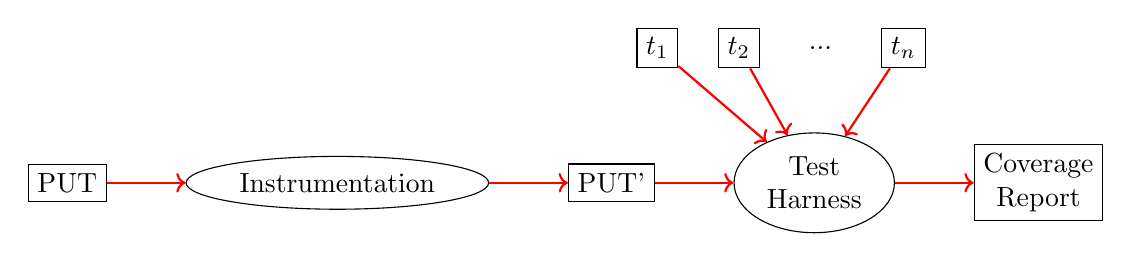
\begin{tikzpicture}
\node[rectangle, draw] (put){PUT};
\node[ellipse, draw, right=of put] (instr){Instrumentation};
\node[rectangle, draw, right=of instr] (putdash){PUT'};
\node[ellipse, draw, align=center, right=of putdash] (th){Test \\ Harness};
\node[rectangle, draw, above left=of th] (t1){$t_1$};
\node[rectangle, draw, right=0.5cm of t1] (t2){$t_2$};
\node[right=0.5cm of t2] (ti){...};
\node[rectangle, draw, right=0.5cm of ti] (tn){$t_n$};
\node[rectangle, draw, align=center, right=of th] (cr){Coverage \\ Report};

\draw[->, Red, thick](put) -- (instr);
\draw[->, Red, thick](instr)--(putdash);
\draw[->, Red, thick](putdash) -- (th);
\draw[->, Red, thick](th)--(cr);
\draw[->, Red, thick](t1) -- (th);
\draw[->, Red, thick](t2) -- (th);
\draw[->, Red, thick](tn) -- (th);
\end{tikzpicture}
\end{center}
\caption{Dataflow architecture}
\label{f:dataflow}
\end{figure}

\begin{figure}[b]
\begin{center}
\begin{tikzpicture}
\node[rectangle, draw, right=of instr] (putdash){PUT'};
\node[rectangle, draw, align=center, right=of putdash] (th){Test \\ Harness};
\node[rectangle, draw, align=center, below=of th] (driver){Driver};
\node[rectangle, draw, align=center, right=3cm of th] (tc){Testcase};
\node[rectangle, draw, align=center, below=of tc](t2){Testcase2};
\node[rectangle, draw, align=center, left=of t2](t1){Testcase1};
\node[align=center, right=of t2](tk){...};
\node[rectangle, draw, align=center, right=of tk](tn){TestcaseN};

\draw[->, dashed] (putdash) -- node[near start, align=center, above]{is \\ aware \\ of}(th); 
\draw[->] (driver)  -- node[near start, left]{executes}(th); 
\draw[Black, arrows={-Triangle[length=0.25cm, width=0.25cm]}]([shift={(0, -0.5)}]tc.south) to (tc);
\draw[-](t1) |- ([shift={(0, -0.5)}]tc.south);
\draw[-](t2) -- ([shift={(0, -0.5)}]tc.south);
\draw[-](tn) |- ([shift={(0, -0.5)}]tc.south);
\draw[->, arrows={-Diamond[length=0.25cm, width=0.25cm]}] (tc.west) -- (th);

\end{tikzpicture}
\end{center}
\caption{Class diagram}
\label{f:class}
\end{figure}

\section{Instrumentation}
The program under test jugs.cpp has been instrumented for
labelling the program locations to be covered with numbers and inserting
logging instruction at these locations. The instrumented version of jugs.cpp
is \lstinline|jugs_instrumented.cpp|.
Testcases and Test harness: The key part of the test automation is implemented
in the file tester.cpp and tester.h. This module implements two classes:
TestHarness provides the capability of running test cases in sequence, recording
and outputing the coverage report. Testcase is the test case class.

\section{Test case Design}
As this is the first cut attempt in getting some hands on experience with unit testing,
we have written the test cases automatically. But, we have followed a somewhat
systematic approach in this. We have drawn a function call graph (doc/dep.dot).
This gives us an idea about the functions which are independent and easier to
test and about those which make calls to other functions. We have chosen to 
first write test cases for testing the functions which are lower down in the
dependency graph (i.e. they are independent).

\begin{figure}
\begin{center}
\includegraphics[width=0.7\textwidth]{images/dep.png}
\end{center}
\caption{Function call graph}
\label{f:fcg}
\end{figure}

\section{Test Cases for Statement Coverage}
Significant statement coverage can be obtained by designing approximately one test case per PUT method. To go further, we need to consider the control flow graphs (CFGs) of the methods to be tested. CFGs are a good starting point to achieve more extensive statement coverage.

\subsection{Control Flow Graphs}
Consider \lstinline[style=jc]|Process::min| method shown in Fig.\ref{f:cfg-min}.

\begin{figure}
\begin{tabular}{c @{} c}
\begin{minipage}{0.4\textwidth}
\begin{lstlisting}[style=jc]
unsigned int Process::min(unsigned int a,
    unsigned int b) {                
  // 50                                                              
  g_testharness.log(50);                                             
  if(a < b) {                                                        
    // 51
    g_testharness.log(51);                                     
    return a;
  }                                                                  
  // 52
  g_testharness.log(52);                                             
  return b;
}              
\end{lstlisting}
\end{minipage}
&
\begin{minipage}{0.6\textwidth}
\begin{center}

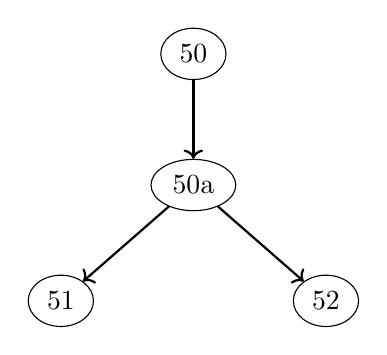
\begin{tikzpicture}
\node[ellipse, draw](50){50};
\node[ellipse, draw, below=of 50](50a){50a};
\node[ellipse, draw, below left=of 50a](51){51};
\node[ellipse, draw, below right=of 50a](52){52};

\draw[->, thick](50) -- (50a);
\draw[->, thick](50a) -- (51);
\draw[->, thick](50a) -- (52);
\end{tikzpicture}
\end{center}
\end{minipage}

\end{tabular}
\caption{Control flow graph: \lstinline[style=jc]|Process::min|}
\label{f:cfg-min}
\end{figure}

\begin{figure}
\begin{tabular}{c @{} c}
\begin{minipage}{0.4\textwidth}
\begin{center}
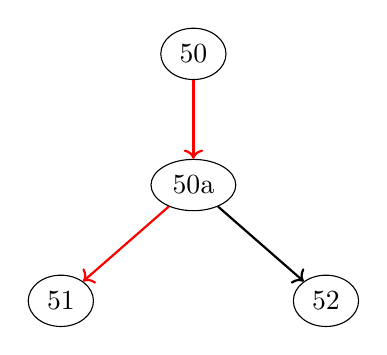
\begin{tikzpicture}
\node[ellipse, draw](50){50};
\node[ellipse, draw, below=of 50](50a){50a};
\node[ellipse, draw, below left=of 50a](51){51};
\node[ellipse, draw, below right=of 50a](52){52};

\draw[->, Red, thick](50) -- (50a);
\draw[->, Red, thick](50a) -- (51);
\draw[->, thick](50a) -- (52);
\end{tikzpicture}
\end{center}
\end{minipage}
&
\begin{minipage}{0.6\textwidth}
\begin{center}
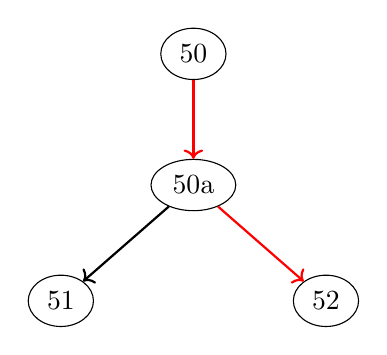
\begin{tikzpicture}
\node[ellipse, draw](50){50};
\node[ellipse, draw, below=of 50](50a){50a};
\node[ellipse, draw, below left=of 50a](51){51};
\node[ellipse, draw, below right=of 50a](52){52};

\draw[->, Red, thick](50) -- (50a);
\draw[->, thick](50a) -- (51);
\draw[->, Red, thick](50a) -- (52);
\end{tikzpicture}
\end{center}
\end{minipage}

\end{tabular}
\caption{Statement coverage: \lstinline[style=jc]|Process::min|}
\label{f:stmt-cov-min}
\end{figure}

\begin{figure}
\begin{center}
\includegraphics[height=0.8\textheight]{images/go-cfg.png}
\end{center}
\caption{Control flow graph: \lstinline[style=jc]|Process::go|}
\label{f:cfg}
\end{figure}

\begin{figure}
\begin{tabular}{c @{} c @{} c}
\begin{minipage}{0.3\textwidth}
\begin{center}
\includegraphics[width=0.9\textwidth]{images/singleStep-cfg1.png}
\end{center}
\end{minipage}
&
\begin{minipage}{0.3\textwidth}
\begin{center}
\includegraphics[width=0.9\textwidth]{images/singleStep-cfg2.png}
\end{center}
\end{minipage}
&
\begin{minipage}{0.3\textwidth}
\begin{center}
\includegraphics[width=0.9\textwidth]{images/singleStep-cfg3.png}
\end{center}
\end{minipage}

\end{tabular}
\caption{Control flow graph: \lstinline[style=jc]|Process::singleStep|}
\label{f:fcg}
\end{figure}

\section{Conclusion}
\subsection{What has been achieved?}
Automated execution of test cases and recording coverage.

\subsection{What next?}
\begin{itemize}
\item Automatic test generation
\item Automated instrumentation
\item Automated function call graph generation


\end{itemize}

\chapter{Automated Test Generation}

\section{Instructions for Use}
To compile the Jugs program, run:
\begin{lstlisting}[style=oc]
	make testgen
\end{lstlisting}

To run the Jugs program, run:
\begin{lstlisting}[style=oc]
	./testgen
\end{lstlisting}

For example, at the time of writing this section, running the above command will yield the following output:
\begin{lstlisting}[style=oc]
PTC_min1 : , 0, 2, 4, 5, 30, 31, 32, 33, 36, 37, 50, 51
PTC_min1 : , 0, 2, 4, 5, 30, 31, 32, 33, 36, 37, 50, 51
PTC_min1 : , 0, 2, 4, 5, 30, 31, 32, 33, 36, 37, 50, 51
PTC_min1 : , 0, 2, 4, 5, 30, 31, 32, 33, 36, 37, 50, 51
PTC_min1 : , 0, 2, 4, 5, 30, 31, 32, 33, 36, 37, 50, 52
test input = , 35005211, 521595368, 294702567, 1726956429, 336465782
test input = , 424238335, 719885386, 1649760492, 596516649, 1189641421
\end{lstlisting}

In the above, we are trying to test the function \lstinline[style=jc]|Process::min|. This function has three statements to be covered which are 50, 51 and 52 (see source file \verb|testgen_main.cpp| to see how this is specified). The first 5 lines show that 5 sets of test inputs were generated before the required coverage was attained. However, only two of these are included in the final output. This is because the test generation algorithm tries to select only those test cases which give us efficient incremental coverage, and throws away those which give no incremental coverage (see Section~\ref{s:tsel} for details).

\section{Random Generation}
Our first attempt at automated test generation is through random generation. The idea is simple, we keep generating test inputs randomly until the desired coverage is achieved. The various components of this problem are as follows:
\begin{enumerate}
\item \textbf{Test input generation:} We create a simple class for this called \lstinline[style=jc]|TestGenerator| that currently generates simple unsigned int values randomly.
\item \textbf{Test setup:} A method/function may require a setup to be tested. This setup has to be done systematically. We assign this responsibility to a abstract class called \lstinline[style=jc]|ParameterisedTestCase|. The primary objective of this class is to abstract away the actual way the input values are fed to the method under test from the \lstinline[style=jc]|TestGenerator| class.
\item \textbf{Coverage data collation:} To keep track of the coverage attained at any point: this problem has already been taken care of in the test harness. We will tweak it a bit and reuse it.
\item \textbf{Test case selection:} The test generator finally tries to come up with an optimised set of test inputs.
\end{enumerate}

\subsection{Architecture}
\begin{figure}
\begin{center}
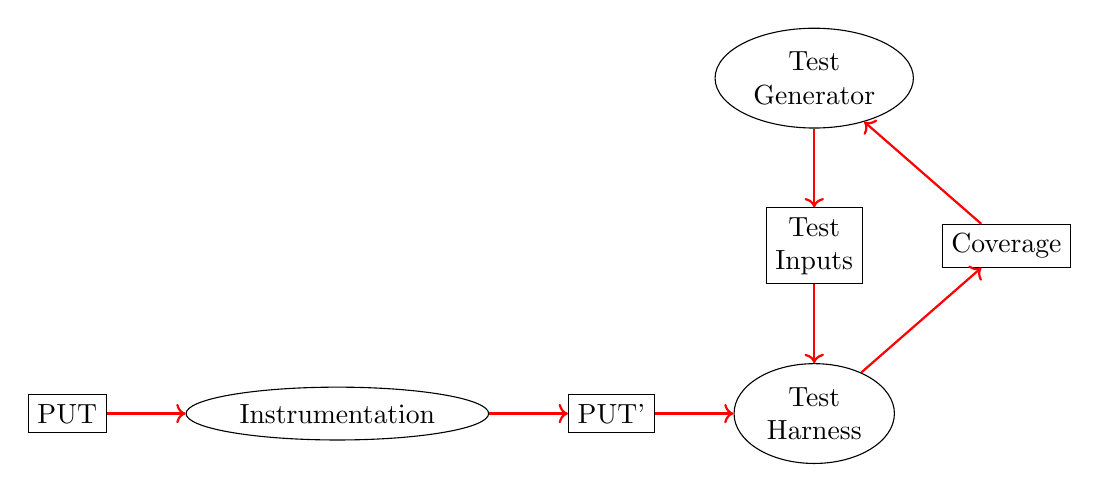
\begin{tikzpicture}
\node[rectangle, draw] (put){PUT};
\node[ellipse, draw, right=of put] (instr){Instrumentation};
\node[rectangle, draw, right=of instr] (putdash){PUT'};
\node[ellipse, draw, align=center, right=of putdash] (th){Test \\ Harness};
\node[rectangle, draw, align=center, above=of th] (ti){Test \\ Inputs};
\node[rectangle, draw, align=center, right =of ti] (cov){Coverage};
\node[ellipse, draw, align=center, above=of ti] (tg){Test \\ Generator};


\draw[->, Red, thick](put) -- (instr);
\draw[->, Red, thick](instr)--(putdash);
\draw[->, Red, thick](putdash) -- (th);
\draw[->, Red, thick](tg) -- (ti);
\draw[->, Red, thick](ti) -- (th);
\draw[->, Red, thick](th) -- (cov);
\draw[->, Red, thick](cov) -- (tg);

\end{tikzpicture}
\end{center}
\caption{Architecture: Random Test Generation}
\label{f:rand-tg-arch}
\end{figure}

\subsection{Test Case Selection} \label{s:tsel}
The total number of tests run before the required coverage is attained may be vastly larger than the actual number of test cases needed to achieve that coverage. Unfortunately, the problem of computing this optimal set of tests is NP-complete. For more details, see set cover problem \cite{Karp1972}. Here, we use a simple heuristic to compute this, shown in Algorithm~\ref{a:tsel}. The algorithm goes through all the test inputs generated and their corresponding coverage. It then iteratively the test input that gives the best incremental coverage of target statements w.r.t. the test inputs selected so far. Please note that this heuristic is a greedy algorithm that does not promise to compute the optimal set. But, this may suffice in many practical cases since having the optimal test input set is neither essential nor feasible in most cases.

\begin{algorithm}
\begin{algorithmic}
\Procedure{selectTestcase}{$T$, $targets$}
\State $T' \gets$ \Call{sort}{$T$} \Comment{Sort in descending order of incremental coverage.}
\State $T'' \gets \{\}$ 
\ForAll{$i \in \{0, ..., |T'| - 1$\}}
	\If{$ct < targets$ \textbf} \Comment{$ct$ -- targets covered}
		\State add $T_i'$ to $T''$
	\EndIf
\EndFor
\State \textbf{return} $T''$
\EndProcedure
\end{algorithmic}
\caption{A basic test selection algorithm}
\label{a:tsel}
\end{algorithm}

\bibliographystyle{alpha}
\bibliography{ref}
\end{document}
